% !TeX spellcheck = en_GB

\documentclass[11pt]{article}
\usepackage{amsmath, alltt, amssymb, xspace, times, epsfig}
\usepackage{amssymb}
\usepackage{graphicx}
\graphicspath{ {images/} }

\setlength{\evensidemargin}{0in} \setlength{\oddsidemargin}{0in}
\setlength{\textwidth}{6.5in} \setlength{\textheight}{8.5in}
\setlength{\topmargin}{0in} \setlength{\headheight}{0in}

\newcommand{\Zn}{\ensuremath{\mathbb{Z}_n}\xspace}
\newcommand{\Zns}{\ensuremath{\mathbb{Z}_n^*}\xspace}
\newcommand{\Zp}{\ensuremath{\mathbb{Z}_p}\xspace}
\newcommand{\Zps}{\ensuremath{\mathbb{Z}_p^*}\xspace}
\newcommand{\Zq}{\ensuremath{\mathbb{Z}_q}\xspace}

\newcommand{\smod}{\ensuremath{\mathrm{mod}\;}}

\newcommand{\DD}{\ensuremath{\mathcal{D}}\xspace}

\newcommand{\Gen}{\ensuremath{\mathsf{Gen}}\xspace}
\newcommand{\Enc}{\ensuremath{\mathsf{Enc}}\xspace}
\newcommand{\Dec}{\ensuremath{\mathsf{Dec}}\xspace}

\renewcommand{\Pr}{\ensuremath{\mathbf{Pr}}\xspace}

\newcommand{\PT}{\ensuremath{\mathsf{PT}}\xspace}
\newcommand{\CT}{\ensuremath{\mathsf{CT}}\xspace}
\newcommand{\Key}{\ensuremath{\mathsf{Key}}\xspace}
\newcommand{\PrivK}{\ensuremath{\mathsf{PrivK}}\xspace}
\newcommand{\eav}{\ensuremath{\mathsf{eav}}\xspace}
\newcommand{\mult}{\ensuremath{\mathsf{mult}}\xspace}

\newcommand{\CC}{\ensuremath{\mathcal{C}}\xspace}
\newcommand{\KK}{\ensuremath{\mathcal{K}}\xspace}
\newcommand{\MM}{\ensuremath{\mathcal{M}}\xspace}
\newcommand{\AAA}{\ensuremath{\mathcal{A}}\xspace}

\newcommand{\sur}[1]{\ensuremath{^{\textrm{#1}}}}
\newcommand{\sous}[1]{\ensuremath{_{\textrm{#1}}}}

\newcommand{\ee}[1]{\ensuremath{#1}}

\newcommand{\note}[1]{\textbf{Note for TA:} #1}\xspace

\begin{document}
%\author{Yiwei Xia}
%\date{}
%\maketitle

\thispagestyle{empty}

\noindent \textbf{COMP 424 \hfill Yiwei Xia}
\begin{center}
{\LARGE notes}
\end{center}

\begin{description}

\item 1 - search problems / uninformed search
\begin{itemize}
	\item notation
	\begin{itemize}
		\item State space \ee{S}: all possible configurations
		\item Initial state \ee{s_0 \in S}: the starting state
		\item Goal states \ee{G \subset S}: the set of end states
		\item Operates \ee{A}: the actions available
		\item Path: the sequence of states
		\item Path cost \ee{c}: number associated with path
		\item Solution: path from \ee{s_0} to \ee{s_g \in G}
		\item Optimal solution: path with minimum cost 
	\end{itemize}
	\item Searching - turn state space into graph
	\subitem vertices are states
	\subitem edges are operators
	\item build a search tree from graph
	\subitem \textbf{search tree nodes are not the same as graph nodes}
	\subitem each node contains a state
	\subitem expand by applying all legal operators, generate successor states
	\item uninformed search - state is not a goal, no idea how far you are from goal
	\subitem moving blindly
		\item properties of search algorithms
	\begin{itemize}
		\item completeness - is finding solution assured
		\item optimality - how good is solution
		\item space complexity
		\item time complexity
	\end{itemize}
	\item search complexity
	\begin{itemize}
		\item branching factor (of state space) - upper limit of how many operators can be applied at any time
		\item solution depth - length of path to shallowest goal state
	\end{itemize}
	\item types of uninformed search
	\begin{itemize}
		\item BFS - FIFO, all nodes at level \ee{i} get expanded before all nodes at level \ee{i + 1}
		\item DFS - LIFO, nodes at deepest level expanded before shallower ones
		\subitem may be better if multiple solutions
		\subitem not guaranteed to terminate
		\item UCS - uniform cost search - BFS doesn't guarantee optimal path if cost per step is non-uniform
		\subitem use priority queue instead of normal queue, add nodes in increasing order of cost of path to node
		\item Depth-limited search - DFS, but terminate if maximum depth allowed is reached
		\item IDS - iterative deepening search - do depth-limited, but increase depth each time solution is not found
		\subitem optimal for problems with unit step costs
		\subitem preferred method for large state space, where solution path unknown
	\end{itemize}

\end{itemize}

\item 2 - informed search
\begin{itemize}
	\item expand based on distance to goal
	\subitem if distance unknown, use heuristic \ee{h(n)}
	\item types of informed search
	\begin{itemize}
		\item Best-first search - expand the most promising node according to heuristic(e.g. smallest Manhattan distance)
		\subitem if heuristic is all 0, best-first = breadth-first
		\subitem UCS is cost so far, best-first is cost to go
		\subitem greedy and suboptimal, does not account for cost so far 
		\item heuristic search
		\subitem adds heuristic (cost to go) + cost so far
		\subitem UCS + best-first search
		\subitem non-optimal, even if it explores all lower heuristic + cost options
		\item \ee{A^*} search - Heuristic search with admissible heuristic
		\subitem optimal + complete
		\subitem exponential worst time, only expands optimal nodes with perfect heuristic
		\subitem can use IDS to save memory
		\item Real-time \ee{A^*} - search a little, choose best path, go down it, search a lil.
		\subitem - backtrack if costs from previous state less than costs in current state
	\end{itemize}
	\item Admissible heuristic
	\begin{itemize}
		\item let \ee{h^*(n)} be shortest path from \ee{n} to any goal state, then:
		\item \ee{h} is admissible if \ee{h(n) \leq h^*(n), \forall n}
		\item h is optimistic, always underestimates cost
		\item solve a relaxed version of problem to obtain admissible heuristic
		\item consistency
		\subitem admissible heuristic is consistent if every successor state \ee{s'}, \ee{h(s) \leq c(s, s') + h(s')}
		\subitem if heuristic of state is \ee{\leq} to heuristic of successor + cost of node to successor
		\subitem monotonic, because cost so far + cost to end is always increasing
		\item if \ee{h_2(n) \geq h_1(n), \forall n}, then \ee{h_2} dominates \ee{h_1}
		\subitem \ee{h_2} is more informative
	\end{itemize}

\end{itemize}

\item 3 - optimization
\begin{itemize}
	\item large combinatorial state space, can't enumerate through all, e.g. travelling salesman, scheduling with durations and mutual constraints, digital circuit layout
	\item described by set of states(=configurations), and an evaluation function
	\item state here means candidate solution, not description of world
	\item state can be partial or incorrect
	\item evaluation function corresponds to path cost
	\item types of search for optimization
	\begin{itemize}
		\item constructive - start from scratch and build a solution e.g. add cities to list of travelling salesman
		\item iterative - start with a broken or suboptimal solution, and improve it e.g. start with city list for travelling
		\item global - start from multiple states that are far apart, go all around the state space 
		\item instead of constructive(informed/uninformed) / iterative(hill-climbing, simulated annealing), global search
\end{itemize}
	
	\item search is local
	\begin{itemize}
		\item previous states(=solutions) are not remembered, apply modification to generate next
	\end{itemize}
	
	\item hill-climbing - go up the hill in graph
	\begin{itemize}
		\item can get stuck in local minimum
		\item randomized hill climbing - instead of picking best move, pick any good move
	\end{itemize}
	
	\item simulated annealing - hill climbing that allows bad moves
	\begin{itemize}
		\item when picking moves, for some probability \ee{p}, accept bad move
		\item pick \ee{p} from boltzmann distribution, \ee{p = e^{-(E-E_i)/T}}, where \ee{T} is temperature, \ee{E} is old value, \ee{E_i} is candidate value
		\begin{itemize}
			\item \ee{T} decreases with every iteration
			\item \ee{T} is high -> exploratory phase, can fuck up a lot
			\item \ee{T} is low -> exploitation phase, trying to find local max
		\end{itemize}
		\item if \ee{T} decreases slowly enough, guaranteed optimal, but may take forever
	\end{itemize}

	\item parallel search - run lots of these in parallel
	
	\item genetic algorithms
	\begin{itemize}
		\item terms
		\begin{itemize}
			\item individual - candidate
			\item fitness
			\item population - set of individuals
			\item individuals change over generations, by applying operations
			\subitem operations = \ee{\{}mutation, crossover, selection\ee{\}}
			\item individuals are binary strings 
		\end{itemize}
		\item elitism - save the best candidate so far on the side so he doesn't accidentally die
	\end{itemize}
	
\end{itemize}

\item 4 - CSP
\begin{itemize}
	\item use constraints to narrow search space
	\item defined by
	\begin{itemize}
		\item variables \ee{V_i} can take values from domain \ee{D_i}
		\item set of constraints specify what combinations of values are allowed (e.g. for subsets of variables, which pairs of variables are allowed)
		\item e.g. \ee{C_1 \neq C_2} or \ee{(C_1 = R, C_2 = G), (C_1 = G, C_2 = R), ...}
		\item typically want any solution, or determine no solution possible
	\end{itemize}
	
	\item approaches for solving CSPs:
	\begin{itemize}
		\item constructive
		\begin{itemize}
			\item state = set of values assigned so far, apply forward search to fill solution
			\item operator = assign value to unassigned variable
			\item depth is limited to number of variables, can use uninformed search e.g. DFS, high branching, many paths lead to same solution
			\item instead, perform \textbf{inference} to reducte search space,
			\item arc-consistent - variable is arc consistent with another if for every permissible value for \ee{v_1} there is a value that \ee{v_2} can take so that the system is still consistent 
			\item generalized arc-consistent - if every value in the domain of every variable is simultaneously arc-consistent
			\item backtracking search - DFS, but fix order of variable assignment
			\begin{itemize}
				\item select unassigned variable, \ee{X}
				\item for each value\ee{=\{x_1,...,x_n\}},
				\subitem if value satisfies constraints \ee{X = x_i}, exit loop
				\item if no assignment, go back to preceding variable and try different value
			\end{itemize}
			\item forward checking - keeep track of legal values for unassigned variables
			\begin{itemize}
				\item when assigning value to variable \ee{X}
				\subitem look at each unassigned variable \ee{Y} connected to \ee{X} by a constraint
				\subitem delete from \ee{Y}'s domain any value that in inconsistent with assignment of \ee{X}
			\end{itemize}
			\item for order of assigning variables
			\begin{enumerate}
				\item pick one with minimum remaining values
				\item pick one that will impose most constraints on remaining variables
				\subitem can use this to break ties of minimum remaining
			\end{enumerate}
		\end{itemize}
	
	
		\item random
		\begin{itemize}
			\item start with broken but complete assignment, gradually fix constraints
			\subitem uses optimization approaches(hill-climbing, simulated annealing)
		\end{itemize}
	
	\end{itemize}

\end{itemize}

\item -5 searching with uncertainty
\begin{itemize}
	\item sources of uncertainty
	\begin{itemize}
		\item non-deterministic actions
		\item unobservable/partially observable state
	\end{itemize}

	\item searching with unobservable states
	\begin{itemize}
		\item belief state
		\subitem a set of currently possible states given actions/observations obtained up to this point
		\subitem usually \ee{2^n} possible beliefs (binary string with every bit being yes no to some variable)
	\end{itemize}

	\item conformant planning
	\begin{itemize}
		\item plan that leads to goal despite uncertainty
		\item heuristic - use actions to narrow down belief to single state, then use standard search
	\end{itemize}

	\item non-deterministic actions
	\item use and/or tree
	\begin{itemize}
		\item or - agent chooses between actions
		\item and - non-deterministic action results induced by environment
		\\ 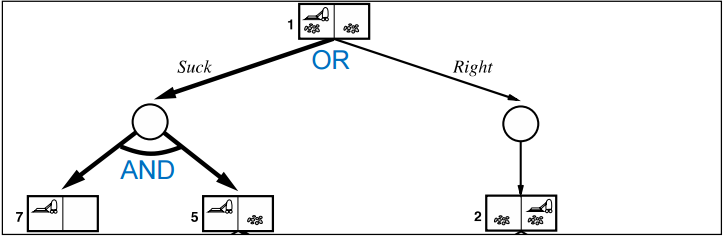
\includegraphics[width=100mm,scale=1]{and_or}
		\item solution is a subtree with
		\begin{itemize}
			\item one action at \textbf{OR} node
			\item includes every outcome at each \textbf{AND} node?
			\item \textbf{has a goal node at every leaf}
		\end{itemize}
	\end{itemize}

	\item partially observable
	\begin{itemize}
		\item include percept, which is noisy evidence about the state
	\end{itemize}
\end{itemize}

\item 6 - games
\begin{itemize}
	\item imperfect information - information is hidden
	\item stochastic - state is partially determined by chance
	\item game search
	\begin{itemize}
		\item definitions
		\begin{itemize}
			\item state - state of board, player turn
			\item operators - legal moves
			\item goal - states in which game is finished(won/lost/draw)
			\item cost - +1 win, -1 lose, 0 draw
			\subitem more complex cases - points won, money won, etc.
			\item utility - prob. of winning or min cost
			\item strategy - way to pick utility moves
		\end{itemize}
		\item minimax
		\begin{itemize}
			\item have two players
			\begin{itemize}
				\item max player - maxes utility - \textbf{UP ARROW}
				\item min player - mins utility - \textbf{DOWN ARROW}
			\end{itemize}
			\item expand complete search tree until all goal states reached and computed
			\item go back up, at each
			\begin{itemize}
				\item min node - pick worst value among children
				\item max node - pick best value among children
				\item intuition - edges below max node are moves it can make, making the nodes below it the board states max-player can turn the board into, which is then min-players turn
			\end{itemize}
			\item if not enough time to enumerate all, go to certain depth, then use evaluation function on end nodes
		\end{itemize}
	
		\item \ee{\alpha}-\ee{\beta} pruning
		\begin{itemize}
			\item if path look worse than what we already had, discard
			\item like minimax, but keeps best leaf for player \ee{\alpha} and opponent \ee{\beta}
			\item use for deterministic, perfect information games
			\item algorithm
			\begin{itemize}
				\item for third layer from the bottom MAX subtree, find the minimum value (the move that MIN will make), then go to next subtree, if there is a min lower, never pick that tree.
				\item have to go all the way down
			\end{itemize}
			\item if branching factor big, search depth limited (Go board game)
			\item optimal only against optimal opponent 
		\end{itemize}
	
		\item forward pruning
		\begin{itemize}
			\item for \ee{\alpha}-\ee{\beta} pruning where the branching factor is too large, evaluate nodes with heuristic before traversing down
			\item PROS
			\begin{itemize}
				\item reduces branching factor
				\item still very good with good heuristic
			\end{itemize}
			\begin{itemize}
				\item can still be suboptimal even with good heuristic
				\item very bad with bad heuristic
			\end{itemize}
		\end{itemize}
	\end{itemize}
\end{itemize}

\item 7 - Monte Carlo tree search
\begin{itemize}
	\item minimax is expensive, needs good evaluation function
	\item random simulations - using randomness to generate samples for estimation is called Monte Carlo method
	\begin{enumerate}
		\item simulate games by randomly selecting moves for both players
		\item keep track of initial move, see who wins
		\item loop n times, pick initial move that has highest win rate
	\end{enumerate}
	\item can split games per move unevenly
	\item MCTS - Monte Carlo Tree Search - combining tree expansion with Monte Carlo simulations
	\begin{enumerate}
		\item \textbf{Selection} - select promising leaves by recursively selecting optimal child nodes using evaluation function(=tree policy)
		\item \textbf{Expansion} - if the leaf in not a terminal node, then create one or more child nodes and select one \ee{C}
		\item \textbf{Simulation} - try possible continuations(=lines) on \ee{C} using default policy. value of move is average of the evaluations from its sampled lines
		\item \textbf{Backpropogation} go back and update values of nodes from the selection/expansion phase
	\end{enumerate}
	\item Monte Carlo Algorithm
	\begin{enumerate}
		\item Descent: select and expand a leaf node in current search tree
		\subitem pick using minimax, or evaluation function
		\item Rollout: when leaf is reached, use Monte Carlo to simulate to end of game or affordable depth
		\item Update: update statistics for all nodes visited during descent by backpropagation
		\item Growth: first state in the rollout is added to tree, and statistics are initialized
	\end{enumerate}
	\item how to choose nodes in Monte Carlo
	\begin{itemize}
		\item exploitaiton - a node seems promising based on previous simulations, explore further
		\item exploration - a node hasn't been played much yet, accrue more information
		\item UCT - upper confidence trees - formula for deciding which node to pick
		\begin{itemize}
			\item use \ee{Q^{\oplus}(s,a) = Q(s,a) + c\sqrt{\frac{\log n(s)}{n(s,a)}}}, pick highest value
			\item \ee{Q(s/a)} value of taking action \ee{a} from state \ee{s}
			\item \ee{n(s,a)} number of times we have taken action \ee{a} from \ee{s}
			\item \ee{n(s)} number of times \ee{s} has been visited in simulations
			\item \ee{c} scaling constant
		\end{itemize}
	\end{itemize}
\end{itemize}

\item 8 - Knowledge Representation and Logic
\begin{itemize}
	\item intelligent agent needs
	\begin{itemize}
		\item perception - what is my state? needs \textbf{recognition}
		\item cognition - what action should i take? needs \textbf{inference}
	\end{itemize}
	\item definitions
	\begin{itemize}
		\item logic - a formal language for representing information from which conclusions can be drawn
		\item syntax - structure, defines what is and isn't allowed as sentence
		\item semantics - meaning
		\item proposition - assertion about the state of the world/game/problem.
		\subitem can be true or false, e.g. today is tuesday
		\item interpretation - assigns true/false value to each proposition
		\item valid - sentence is valid if true in all interpretations are true
		\item satisfiable - sentence is valid for some interpretation
		\item unsatisfiable - false for all interpretations
		\item knowledge base KB entails sentence \ee{\alpha} iff \ee{\alpha} is true in all worlds where KB is true
		\subitem KB \ee{\vDash \alpha}
		\item CNF - conjunctive normal form
		\subitem \ee{(x_1 \vee x_2) \wedge (x_2 \vee x_3)}
		\item DNF - disjunctive normal form
		\subitem \ee{(x_1 \wedge x_2) \vee (x_2 \wedge x_3)}
		\item Horn form - conjunction, clauses with \ee{\leq 1} positive literal 
		\subitem \ee{(x_1 \vee \lnot x_2) \wedge (x_1 \vee \lnot x_2 \vee \lnot x_3)}
		\subitem same as \ee{x_2 \implies x_1} and \ee{x_2 \wedge x_3 \implies x_1}
	\end{itemize}
	\item inference rules for propositional logic
	\begin{itemize}
		\item forward chaining
		\begin{itemize}
			\item when new sentence \ee{p} is added to KB
			\begin{itemize}
				\item look for all sentences that share literals with \ee{p}
				\item perform resolution
				\item add new sentences to KB and continue
			\end{itemize}
		\end{itemize}
	
		\item backward chaining
		\begin{itemize}
			\item when a query \ee{q} is asked of the KB
			\begin{itemize}
				\item if \ee{q} already in the KB, return true
				\item else use resolution for \ee{q} with other sentences in the KB, and continue from the result
			\end{itemize}
			\item backward chaining is goal driven, centers around query being asked
			\item lazy evaluation - new facts are only inferred as needed, and only to the extent that they help answer the question
		\end{itemize}
	\end{itemize}
\end{itemize}

\item 9 - first order logic
\begin{itemize}
	\item propositional logic is too simple
	\item elements
	\begin{itemize}
		\item predicates - used to describe objects, properties, relationships
		\item quantifiers - \ee{\forall} = for all, \ee{\exists} = there exists, used for statements that apply to class of objects
		\item functions - used to give you an object that is related to another object in a specific way
		\subitem these objects (domain elements) are drawn from domain
		\item e.g. \ee{\forall x}On\ee{(x,}Table\ee{) \rightarrow}Fruit\ee{(x)}
		\begin{itemize}
			\item \ee{\forall} is a quantifier
			\item \ee{x} is variable
			\item Table is constant
			\item On is a predicate
			\item Fruit() is function
			\item \ee{\rightarrow} is a connective
			\subitem so is \ee{\wedge}, \ee{\vee}, \ee{\lnot}, etc.
		\end{itemize}
		\item be careful! \ee{\exists x.} Taking\ee{(x,}AI\ee{)\rightarrow}Smart\ee{(x)} is equivalent to \ee{\exists x.\lnot}Taking\ee{(x,}AI\ee{)\vee}Smart\ee{(x)}, so if anyone is not taking AI, that statement is still true. Don't use \ee{\rightarrow} with \ee{\exists}
		\item quantifier duality
		\begin{itemize}
			\item \ee{\forall x Loves(x,IceCream) = \lnot \exists x \lnot Loves(x, IceCream)} 
			\item \ee{\exists x Loves(x, Broccoli) = \lnot \forall x \lnot Loves(x, Broccoli)}
		\end{itemize}
		
		\item sentences are true with respect to a \textbf{model}
		\item model \ee{M = (D,I)}, where 
		\begin{itemize}
			\item \ee{D} is a domain of objects
			\item \ee{I} is an interpretation
			\begin{itemize}
				\item constant symbols \ee{\rightarrow} objects
				\item predicate symbols \ee{\rightarrow} relations over objects
				\item function symbols \ee{\rightarrow} functional relations over objects
			\end{itemize}
		\end{itemize}
		
		\item inference algorithms for FOL(very expensive)
		\begin{enumerate}
			\item Propositionalize the FOL into propositional logic - too expensive
			
			\item search - search using operators that work in FOL
			\begin{itemize}
				\item Modus Ponens (MP) - if \ee{\alpha}, and \ee{\alpha \rightarrow \beta}, then \ee{\beta}
				\item And-Introduction - if \ee{Cool(Joe)} and \ee{CSMajor(Joe)} in KB, then \ee{Cool(Joe) and CSMajor(Joe)}
				\item Universal Elimination - if \ee{\forall x. Takes(x, AI) \rightarrow Cool(x)}, then \ee{Takes(Pat,AI) \rightarrow Cool(Pat)}
				
				\item use pattern matching to find promising candidates for UE
				\item use a substitution to make two sentences the same
				\\ 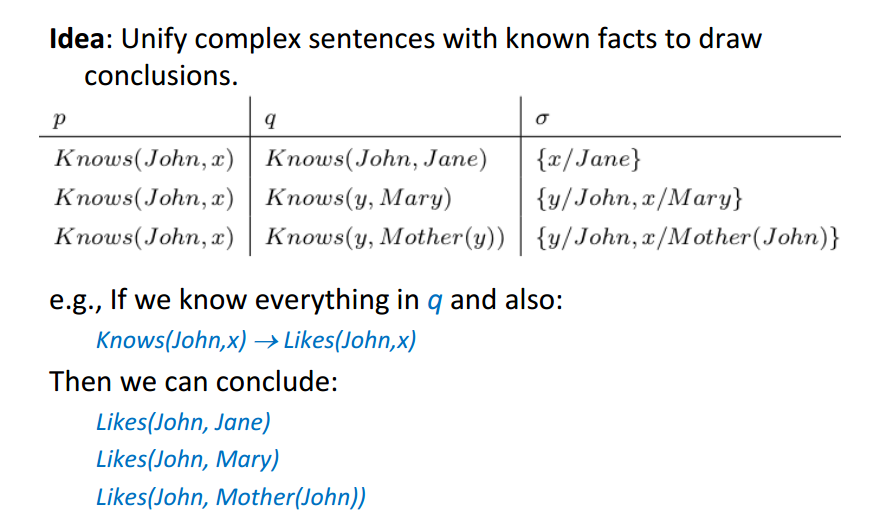
\includegraphics[width=100mm,scale=1]{unification}
				\item like solving a system of equations with logic
				
				\item generalized modus ponens
				\begin{itemize}
					\item if we have \ee{p_1', p_2',...p_n'}, and \ee{(p_1 \wedge p_2 \wedge ... \wedge p_n \rightarrow q)}, then \ee{q\sigma}, where \ee{p_i'\sigma = p_i \sigma}
				\end{itemize}
				
			\end{itemize}
		
			\item resolution
			\begin{itemize}
				\item pretty much if \ee{p \vee q} and \ee{\lnot q \vee r}, then \ee{p \vee r}
	
			\end{itemize}
	
		\end{enumerate}
	\end{itemize}
\end{itemize}

\item 10 - Planning
\begin{itemize}
	\item plan - collection of actions to perform a task
	\item STRIPS
	\begin{itemize}
		\item domain - set of typed objects represented by propositions
		
		\item states - represented as first order predicates over objects
		\begin{itemize}
			\item e.g. \ee{In(robot, room) \wedge Closed(door) \wedge ...}
			\item closed world assumption
			\subitem everything not stated is false
			\subitem only objects in the world are the ones that are defined
			\item goals are states
		\end{itemize}
	
		\item operators - defined in terms of
		\begin{itemize}
			\item preconditions - when can the action be applied - conj. of literals
			\item effects - what happens after the action?
			\item predicates as well
		\end{itemize}
	
		\item action schema
		\begin{itemize}
			\item way to define operator as an ordered triplet
			\item \ee{\{Name,Preconditions,Effects\}}
			\item effects and postconditions are expressed as
			\begin{itemize}
				\item add-list - list of propositions that become true after action
				\item delete-list - list of propositions that become false after action
				\item e.g. \ee{At(robot,y) \wedge \lnot At(robot,x)}
			\end{itemize}
		\end{itemize}
	
		\item semantics
		\begin{itemize}
			\item if precondition is false in world state, then action does not change anything
			\begin{itemize}
				\item action does not get applied at all
			\end{itemize}
			\item if precondition is true, \textbf{IN THIS ORDER}, delete items in delete-list, add items in add-list
		\end{itemize}
	
		\item pros
		\begin{itemize}
			\item restricted, low branching, efficient inference
			\item all operations are adding or deleting from KB
		\end{itemize}
	
		\item cons
		\begin{itemize}
			\item limited, assumes small number props per action
		\end{itemize}
	
		\item approaches to planning
		\begin{itemize}
			\item states-space planning - uses states and operators
			\begin{itemize}
				\item finding plan is constructive search through state space for goal states
			\end{itemize}
			
			\item plan-space planning - partial order planning - R\&N 10.4.4
		\end{itemize}
	
		\item state-space planning
		\begin{itemize}
			\item forward planning
			\begin{enumerate}
				\item basic idea - reason from start state, try to find operators that can be applied
				\item determine all operators that work on start state
				\item ground operators - replace variables with any combinations of constants
				\item choose a grounded operator to apply
				\item determine new content of KB, based on operator
			\end{enumerate}
			
			\item regression planning
			\begin{enumerate}
				\item basic idea - reason from goal state, find the actions that will lead to goal
				\item pick some actions \ee{A} that satisfy some of the goals
				\item make a new goal, adding preconditions of \ee{A} to set of propositions
				\item repeat until goal set is satisfied by start state
			\end{enumerate}
		\end{itemize}
	
		\item STRIPS attributes
		\begin{itemize}
			\item sound - only legal plans will be found
			\item - not complete - once subgoal ordering is selected, no backtracking
			\item suboptimal - no guarantee of finding shortest plan
			\item expensive - usually NP-hard or worse
		\end{itemize}
	
		\item other solutions
		\begin{itemize}
			\item SATPlan - satisfiablity problem
			\item Heuristic search
			\item GraphPlan
			\item Fast forward planning - use hill climbing approximate, then best-first
			\item Hierarchal task network - decompose complex planning into hierarchy of smaller planning problems
		\end{itemize}
	\end{itemize}
\end{itemize}


\item 11 - uncertainty
\begin{itemize}
	
	\item problems with planning
	\begin{itemize}
		\item incomplete information
		\begin{itemize}
			\item unknown predications (states)
			\item disjunctive effects i.e. either A or B happens when operator happens
		\end{itemize}
	
		\item incorrect information
		\begin{itemize}
			\item current state incorrect
			\item unanticipated outcomes (missing/incorrect postconditions for operators), makes whole plan incorrect
		\end{itemize}
	
		\item qualification problem
		\begin{itemize}
			\item all required preconditions + possible condition outcomes combinatorially huge
		\end{itemize}
	\end{itemize}

	\item solutions
	\begin{itemize}
		\item conditional (contingency) planning
		\begin{itemize}
			\item include observation actions, chick if things are okay, contingency plans if not okay
			\item expensive, because gotta cover all the things that can go wrong
		\end{itemize}
	
		\item monitoring/replanning
		\begin{itemize}
			\item assume normal states/outcomes
			\item check progress during execution, try again if failed
		\end{itemize}
	
		\item solutions are either implicit or explicit
		\begin{itemize}
			\item implicit
			\begin{itemize}
				\item avoid it, make plan that is robust to it, uncertainty doesn't make problems
			\end{itemize}
		
			\item explicit
			\begin{itemize}
				\item build a model to describes it, and deal with it
				\item describing using logic is not robust - risks falsehoods, and leads to weak conclusions
				\item use Bayesian probability!

			\end{itemize}
		\end{itemize}
	
		\item Bayesian probability
		\begin{itemize}
			\item best waifu for dealing with uncertainty
			\item clear semantically + intuitive, can be learned from data
			\item definitions
			\begin{itemize}
				\item belief - a belief relates a logical proposition to current state of knowledge/current state of world
				\item beliefs are subjective, based on one's state of knowledge, and different agents may hold different beliefs
			\end{itemize}
		
			\item new evidence changes probabilities of propositions
			
			\item prior (unconditional) beliefs denote belief before the arrival of any evidence
			
		\end{itemize}
	
		\item decision theory = utility theory + probability theory

		\item probability theory
		\begin{itemize}
			\item pretty much just normal probability things
			\item define the world as set of random variables
			\item world is divided into a set of elementary, mutually exclusive events(=states)
			\item probabilistic model - allows us to compute probabilities of any event in world
			\item joint probability distribution - assigns weights to each event
			\item unconditional probability = sum of all entries from joint distribution
		\end{itemize}
	
		\item Bayes Rule - \ee{P(H \mid e) = P(e \mid H) P(H)/P(e)}
		\begin{itemize}
			\item \ee{P(H\mid e)} - posterior probability
			\item \ee{P(H)} - prior probability
			\item \ee{P(e\mid H) }- likelihood
			\item \ee{P(e)} - normalizing constant
			\subitem \ee{P(e) = P(e \mid H) P(H) + P(e \mid ~H) P(~H)}
		\end{itemize}
	\end{itemize}
\end{itemize}

\item 12 - bayesian networks
\begin{itemize}
	\item represent conditional independence using graph model
	\\ 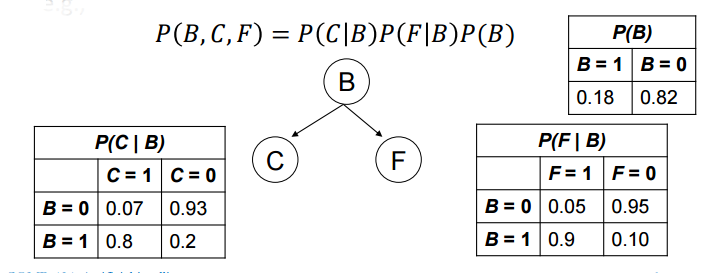
\includegraphics[width=100mm,scale=1]{bayes_net}
	\item \ee{P(C \vert B)}, then \ee{B \rightarrow C}
	\item one node for each variable in problem
	\item arcs(=arrows) are direct influences
	\begin{itemize}
		\item 
	\end{itemize}
\end{itemize}

\end{description}

\end{document}
 